\documentclass[titlepage]{article}
% preamble area, where packages used
\usepackage{amsmath} % package usage example

% paper setting
\setlength{\textwidth}{16.0cm}
\setlength{\textheight}{22.0cm}
\setlength{\oddsidemargin}{0.0cm}
\setlength{\topmargin}{0.0cm}

% ****paragraph and line setting****
% paragraph indentation
\setlength\parindent{0ex}
% paragraph skip: baselineskip=fontsize * baselinestretch, where fontsize is a constant corresponding to a chosen font type.
\setlength{\parskip}{0.5\baselineskip}
% line skip
\renewcommand{\baselinestretch}{1.5}

\usepackage{hyperref}
\usepackage[section,nottoc]{tocbibind}

\usepackage{graphicx}
\usepackage{rotating}
% declare the path(s) where your graphic files are
\graphicspath{{./fig/}}
% and their extensions so you won't have to specify these with
% every instance of \includegraphics
\DeclareGraphicsExtensions{.png}

\usepackage{amsmath}
\numberwithin{figure}{section}
\numberwithin{equation}{section}

\usepackage{algpseudocode}
\usepackage{algorithm}

\usepackage{listings}

\usepackage{comment}

\usepackage{xeCJK}
\setCJKmainfont{WenQuanYi Micro Hei Mono}

\begin{document}

\title{ParWiBench Internal}
\author{Xuechao Wei}
\date{\today}
\maketitle


% main text

\section{LTE Background}

\textbf{Frame structure}\cite{erik}

The size of various fields in the time domain is expressed as a number of time units $T_{s}=1/(15000*2048)$.

Downlink and uplink transmissions are organized into radio frames with $T_{f}=3072000*T_{s}=10ms$ duration.

\textbf{Frame structure type 1}

$T_{f}=3072000*T_{s}=10ms$ long and consists of 20 slots of length $T_{slot}=15360*T_{s}=0.5ms$, numbered from 0 to 19. A subframe is defined as two consecutive slots where subframe $i$ consists of slots $2i$ and $2i+1$.

\textbf{TTI}

Data on a transport channel is organized into transport blocks. In each Transmission Time Interval (TTI), at most one transport block of a certain size is transmitted over the radio interface to/from a mobile terminal in absense of spatial multiplexing. In case of spatial multiplexing (MIMO), there can be up to two transport blocks per TTI.

Associated with each transport block is a Transport Format (TF), specifying how the transport block is to be transmitted over the radio interface. The transport format includes information about the transport-block size, the modulation scheme, and the antenna mapping. Together with the resource assignment, the resulting code rate can then be derived from the transport format. By varying the transport format, the MAC layer can thus realize different data rates. Rate control is therefore also known as transport-format selection.

LTE has inherited the basic principle of WCMA/HSPA that data are delivered to the physical layer in the form of Transport Blocks of a certain size. In terms of the more detailed transport-block structure, LTE has adopted a similar approach as was adopted for HSPA:

\subsection{LTE Downlink Scheme}

\textbf{Modulation}

如果想要传输一串输入数字信号(二进制bit流),就必须把这些信号放到正弦波上,因为无线信号在空气中是通过正弦波传输的,所以在把信号放到正弦波上以后,正弦函数的一些参量如振幅、频率、相位均可用来体现不同的信号值。

例如,如果正弦波的函数是

\begin{equation}
C*cos(f_{c}*t+\phi)
\end{equation}

以QAM为例,将上式展开一下化为

\begin{equation}
A*cos(f_{c}*t)+B*sin(f_{c}*t)
\end{equation}

现在希望将输入信号由A和B携带,这时就同时利用了振幅和相位来携带信息。如果A和B携带两个bit的信息,那么可以建立一个每两bit和一个实数的映射关系:

\begin{verbatim}
01-->1
10-->3
11-->-1
00-->-3
\end{verbatim}

如果将每两个实数分别作为一个复数的实部和虚部,那么一个复数就可以表示4bit的信息。进一步,如果将这个复数的实部和虚部分别对应于上面第2个式子中的A和B,那么就可以将每4bit的信息映射到一个正弦波上,这就完成了正弦波的信息携带。

我们需要做的只是一个映射工作,然后将每个复数的实部和虚部发送到发射电路,电路会完成“载波”的任务。相反,在接受端也会有一个滤波电路,将接受到的正弦波的A和B解出来然后发送给后面的解调及解码过程。

\textbf{OFDM}

OFDM的目的是将n个经过调制的频域信号转化为n个时域信号,每一个时域信号都由一系列间隔为$\Delta f$的子载波叠加而成,这些子载波相互正交。时域信号实际上是由n个频域信号时域化后采样得到。

假设经过基带调频并经过电路调制到高频之后,在$[0,T_{u}]$时间内,第$i$个子载波上已调的QAM信号可以表示为

\begin{equation}
	s_{i}(t)=A_{i_{c}}g(t)cos(2\pi f_{i}t)-A_{i_{s}}g(t)sin(2\pi f_{i}t)
=Re\{[A_{i_{c}}+jA_{i_{s}}]g(t)e^{j2 \pi f_{i}t}\}
=Re\{A_{i}g(t)e^{j2 \pi f_{i}t}\}
\end{equation}

其中,$A_{i}=A_{i_{c}}+jA_{i_{s}}$是发送的QAM符号的星座点,$A_{i_{c}}$和$A_{i_{s}}$分别是其同相分量(I路)和正交分量(Q路);$f_{i}=f_{c}+i\Delta f=f_{c}+{i\over T_{u}}$是第$i$路的载波频率,$i=0,1,...,N-1$;$g(t)$是脉冲成形滤波器的冲激响应,假设它为矩形脉冲。

总的OFDM信号可以表示为

\begin{equation}
	s(t)=\sum _{i=0} ^{N-1}s_{i}(t)
	=Re\{[\sum A_{i}g(t)e^{j{2 \pi}i{\Delta f}t}]e^{j{2 \pi}f_{c}t}\}
	=Re\{a(t)e^{j{2 \pi}f_{c}t}\}
\end{equation}

其中

\begin{equation}
	a(t)=\sum _{i=0}^{N-1}A_{i}g(t)e^{j{2\pi}i{\Delta f}t}
\end{equation}

是OFDM信号的复包络。

若令$I(t)=Re\{a(t)\}$,$Q(t)=Im\{a(t)\}$,则$s(t)$可以表示为

\begin{equation}
	s(t)=I(t)cos(2 \pi f_{c}t)-Q(t)sin(2 \pi f_{c}t)
\end{equation}

因此也可以先得到复包络$a(t)$,再经过I/Q\textbf{正交调制}来得到OFDM信号。

需要注意的是,对于BPSK、MASK这样的一维调制,所考虑的载波是$cos(2\pi f_{i}t)$,已调信号只有同相载波,没有正交载波$sin(2 \pi f_{i}t)$,因此载波正交的最小间隔是$1\over {2T_{u}}$,而不是$1\over {T_{u}}$。要保证同相载波和正交载波同时都正交,这就需要载波间隔为$1\over T_{u}$。由$s_{i}t$可见,对于二维调制,I路和Q路这两个载波可以表示为一个复数载波$e^{j2\pi f_{i}t}$(这里还不太理解)。对于两个复载波$c_{n}=g(t)e^{j2\pi f_{n}t}$和$c_{m}=g(t)e^{j2\pi f_{m}t}$,假设$g(t)$为矩形脉冲,则使$c_{n}(t)$和$c_{m}(t)$保持正交的最小间隔是$|f_{n}-f_{m}|=1\over T_{u}$。

为了实现OFDM调制的基带数字处理,首先要将OFDM信号的复包络进行采样,成为离散时间信号。

在$[0,T_{u}] (T_{u}={1\over {\Delta f}})$,$T_{u}=N*T_{samp}$,$T_{samp}$为采样频率的倒数。如果$N=2048$且$\Delta f = 15KHz$,则$T_{samp}=T_{s}$,$T_{s}$为time unit\cite{erik},大小为$1/(15000*2048)$。若采样时刻是$m{T_{u} \over N}, m=0,1,...,N-1$,则对OFDM信号的复包络$a(t)$采样后的序列为

\begin{equation}
	a_{m}=a(m{T_{u}\over N})=\sum _{i=0} ^{N-1} A_{i}e^{j2\pi i \Delta f m{T_{u} \over N}}
	=\sum _{i=0} ^{N-1}A_{i}e^{j2\pi {mi \over N}} \ m = 0,1,...,N-1
\end{equation}

该式恰好就是对序列$\{A_{0},A_{1},...,A_{N-1}\}$进行离散傅里叶反变换(IDFT)的结果。其中,IDFT得到的$N$个时间间隔为$T_{samp}$的一组输出叫做一个OFDM符号(OFDM symbol)。因此,给定输入的符号$\{A_{0},A_{1},...,A_{N-1}\}$后,借助IDFT即可得到OFDM复包络的时间采样。

接收端通过I/Q正交解调后可以恢复OFDM信号的复包络$a(t)$,将其采样得到的时间序列$\{a_{m}\}=\{a_{0},a_{1},...,a_{N-1}\}$。由于IDFT是可逆变换,因此对序列$\{a_{m}\}$进行离散傅里叶变换(DFT)即可得到发送的序列$\{A_{i}\}$:

\begin{equation}
	A_{i}=\sum _{m=0} ^{N-1}a_{m}e^{-j2\pi {mi\over N}} \ i = 0,1,...,N-1
\end{equation}

由于$\{a_{m}\}$是对时间信号的采样,故称其为时域序列。而$\{A_{i}\}$是序列$\{a_{m}\}$的离散傅里叶变换,故称其为频域序列。

当$N$为2的整幂时,DFT和IDFT存在快速算法:FFT和IFFT。这样,可以借助FFT和IFFT来实现OFDM信号的调制与解调。

\textbf{[Aside: ]}对\textbf{正交}、\textbf{频分}和\textbf{复用}的理解

我觉得\textbf{正交}包含两方面的含义,一指构成每个OFDM符号的各子载波彼此正交;二指往高频调制时,正交调制器附加的同相载波和正交载波相互正交。前者我需要关心,后者由调制电路来做,我不用管;\textbf{频分}是指各子载波的频率间隔为$\Delta f$;感觉\textbf{复用}最难理解,理想的正弦波的频谱其实是单值函数,即只在一个频率处有非零值,其它频率处都为0。但实际上由计算机生成的正弦波都是锯齿状的,看起来由许许多多的台阶构成,这就使得实际的“正弦波”频谱图如图2中的任意一个子载波所示,图中最高波峰即为我们所需要的理想正弦波频谱的那个非零值。传统的FDM做法是让每个子载波间隔足够大的$\Delta f$值,使得每个子载波的最大频谱波形彼此分开,如图1所示。而OFDM则保证只要用一个最小的$\Delta f$使子载波正交,就可以用如下函数将各子载波的最大非零频谱值区分出来(虽然彼此之间存在重叠干扰):

\begin{equation}
	s(f)=\left\{
		\begin{array}{ll}
			0 & \textrm{if $f=n\Delta f (n \neq 0)$} \\
			a_{0}+b_{0}j & \textrm{else}
		\end{array}
		\right.
\end{equation}

\begin{figure}[htbp]
	\centering
	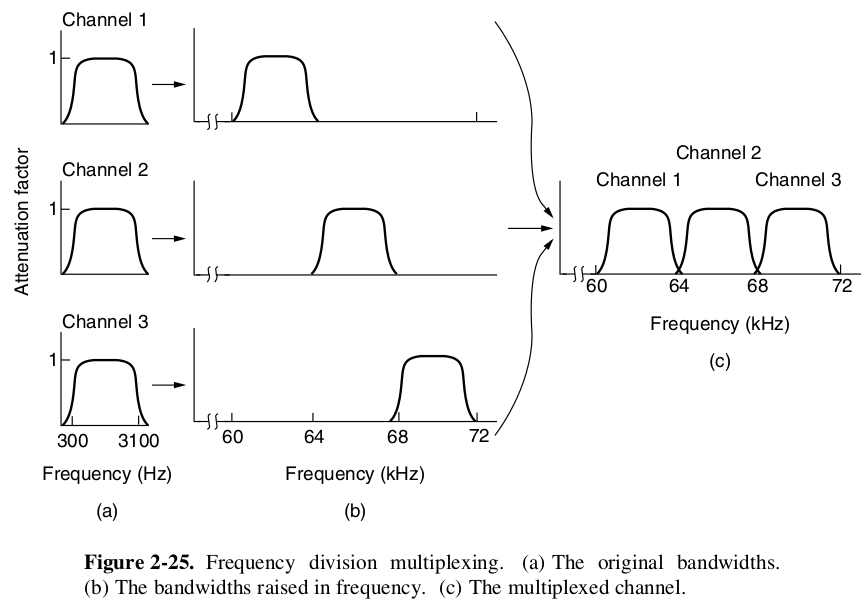
\includegraphics[height=3.14159in]{FDM}
	\caption{Traditional FDM}
\end{figure}

\begin{figure}[htbp]
	\centering
	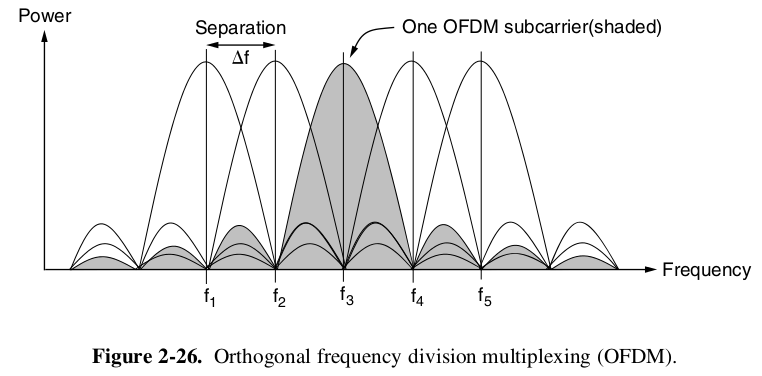
\includegraphics[height=2.5in]{OFDM}
	\caption{OFDM}
\end{figure}

当然,这只是非常粗略理解。

\textbf{CRC}

循环冗余校验是通过模2除法运算来建立有效信息位和校验位之间的约定关系。其中待编码的有效信息以多项式$M(x)$表示,将它左移若干位后,用另一个约定好的多项式$G(x)$去除,所产生的余数就是校验位。当接受方收到发来的CRC码后,他仍用约定的$G(x)$去除,若余数为0,表明该代码接受无误;若余数不为0,表明某一位出错,再进一步由余数值确定出错的位置,并予以纠正。

CRC的编码步骤如下:

\begin{itemize}
	\item 将待编码的$N$位有效信息位表示为一个$n-1$阶的多项式$M(x)$;
	\item 将$M(x)$左移$K$位,得到$M(x)x^{k}$($k$由预选的$k+1$位的生成多项式$G(x)$决定);
	\item 用一个预选好的$k+1$位的生成多项式$G(x)$对$G(x)x^{k}$做模2除法;
	\item 把左移$k$位后的有效信息位与余数做模2加法,即形成长度为$N+K$的CRC码。
\end{itemize}

\textbf{Turbo coding}

The transfer function of the 8-state constituent code for the PCCC (Parallel Concatenated Convolutional Code) is\cite{36series-212}:

\begin{displaymath}
	G(D)=[1,{g_{1}(D) \over g_{0}(D)}]
\end{displaymath}

where

\begin{displaymath}
	g_{0}(D)=1+D^{2}+D^{3} \\
	g_{1}(D)=1+D+D^{3}
\end{displaymath}

\begin{figure}[htbp]
	\centering
	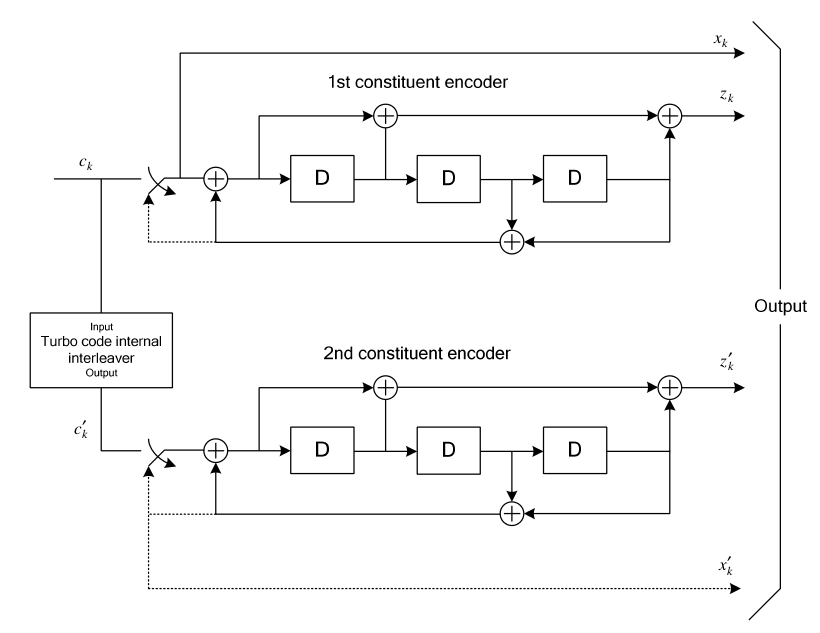
\includegraphics[height=3in]{turbo}
	\caption{Structure of rate 1/3 turbo encoder (dotted lines apply for trellis termination only)}
\end{figure}

\begin{itemize}
	\item In case of single-antenna transmission there is a single transport block of dynamic size for each TTI.

	\item In case of multi-antenna transmission, there can be up to two transport blocks of dynamic size for each TTI, where each transport block corresponds to one codeword in case of downlink spatial multiplexing. This implies that, although LTE supports downlink spatial multiplexing with up to four layers, the number of codewords and thus also the number of transport blocks is still limited to two.
\end{itemize}

\textbf{Channel mapping}

\begin{figure}[htbp]
	\centering
	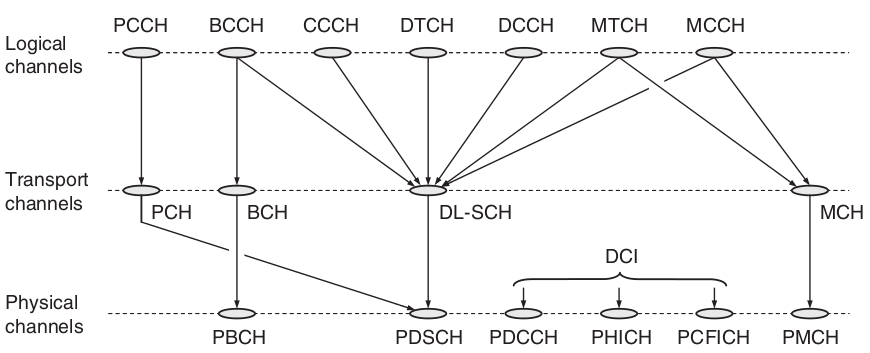
\includegraphics[height=2in]{DLCH}
	\caption{Downlink channel mapping}
\end{figure}

\begin{figure}[htbp]
	\centering
	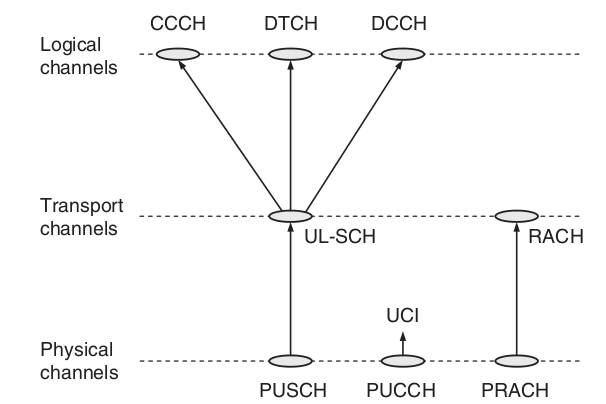
\includegraphics[height=2.2in]{ULCH}
	\caption{Uplink channel mapping}
\end{figure}

我对channel mapping的概念感到极其不理解,但从下面的文字中貌似可以看出transport channel和physical channel的联系:

To the transport block(s) to transmit on the DL-SCH, a CRC, used for error detection in the receiver, is attached, followed by Turbo coding for error correction. In case of spatial multiplexing, the processing is duplicated for each of the transport blocks. Rate matching is used not only to match the number of coded bits to the amount of resources allocated for the DL-SCH transmission, but also to generate the different redundancy versions as controlled by the hybrid-ARQ protocol.

After rate matching, the coded bits are modulated using QPSK, 16QAM, or 64QAM, followed by antenna mapping. The antenna mapping can be configured to provide different multi-antenna transmission schemes including transmit diversity, beam-forming, and spatial multiplexing. Finally, the output of the antenna processing is mapped to the physical resources used for the DL-SCH. The resources, as well as the transport-block size and the modulatin scheme, are under control of the scheduler.

A \textit{phsical channel} corresponds to the set of time-frequency resources used for transmission of a particular transport channel and each transport channel is mapped to a corresponding physical channel.

经过师兄的指点,现在的理解是,物理信道主要负责资源块的分配,传输信道负责前面的编码部分。

\textbf{The downlink physical resource}

\begin{figure}[htbp]\label{fig:res-grid}
	\centering
	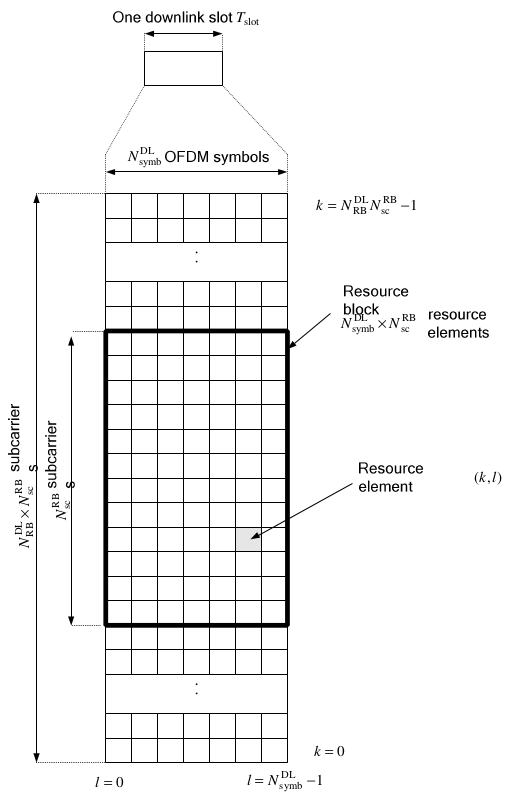
\includegraphics[height=4.5in]{res-grid}
	\caption{LTE downlink resource grid\cite{36series-211}}
\end{figure}

\begin{figure}[htbp]\label{fig:phy-params}
	\centering
	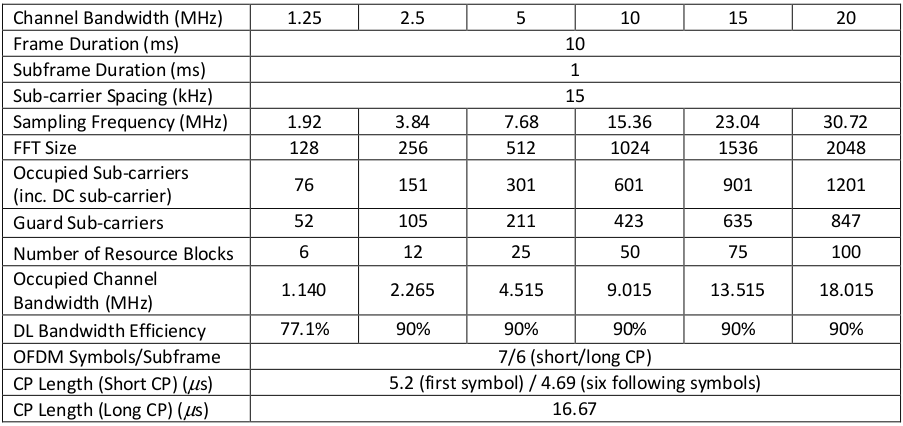
\includegraphics[height=2.5in]{phy-params}
	\caption{LTE downlink physical layer parameters\cite{nutshell}}
\end{figure}

\begin{figure}[htbp]
	\centering
	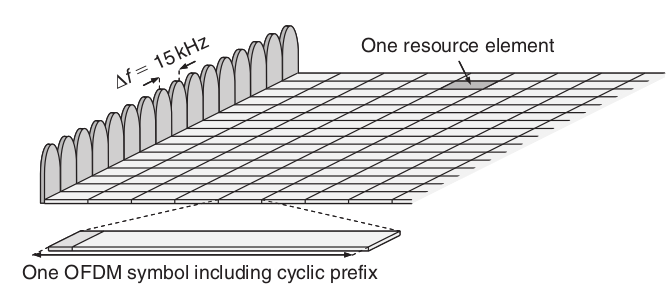
\includegraphics[height=1.5in]{DL-PHY-RES}
	\caption{LTE downlink physical resource}
\end{figure}

\begin{figure}[htbp]
	\centering
	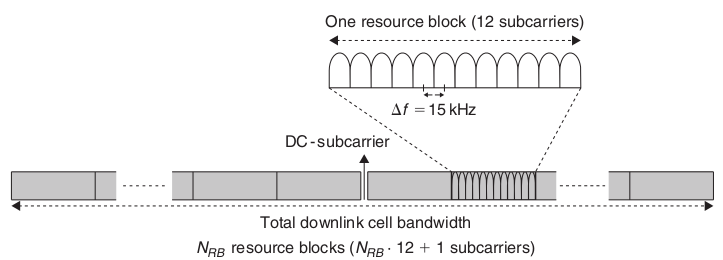
\includegraphics[height=1.5in]{DL-Frequency}
	\caption{Frequency-domain structure for LTE downlink}
\end{figure}

\begin{figure}[htbp]\label{fig:DL-Time}
	\centering
	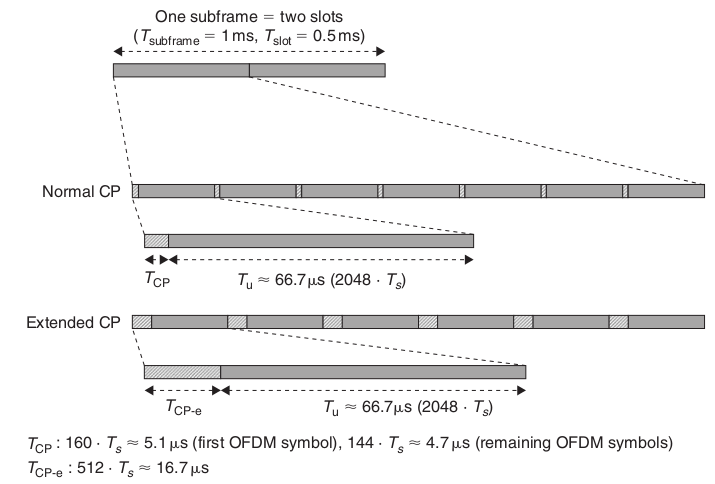
\includegraphics[height=3in]{DL-Time}
	\caption{Detailed time-domain structure for LTE downlink transmission}
\end{figure}

\begin{comment}
\section{LTE Downlink Simulator}
\end{comment}

\section{Benchmark Suite Implementation}

\subsection{Frame Parameters}

\textbf{Downlink}

\textbf{Uplink}

一帧处理的bit长度是由LTE资源块的大小决定的,而资源块的大小由采样频率决定。因此一旦采样频率确定,通过从后往前推,各个模块能够处理的最大数据长度及其至少应该达到的throughput也就是确定的。

由于Uplink和Downlink使用的资源块结构相同,因此上行PHY层每帧的参数信息也可以参考\ref{fig:phy-params}。与下行不同,以Tx为例,上行在进入resource mapping之前要先经过一次DFT,因此在resouce mapping之前的模块,其参数与DFT的长度有关,而不是IFFT的长度。

下面以resouce mapping为界、采样频率为15.36MHz来计算各个模块的输入输出数据长度以及模块的throughput。

\ref{fig:res-block}是\ref{fig:res-grid}和\ref{fig:DL-Time}的结合,表示子帧(slot或subframe)结构,一帧中包含两个子帧。其中水平方向的长度NumULSymbSF表示一个子帧中的OFDM符号数目,目前为常数14。垂直方向的长度为子载波的数目,是与带宽对应的量,例如带宽为1.25MHz时,子载波的数目为76,这个值只有在发射端和接收端的前端才会起作用,而对于Tx和Rx的baseband处理时我们不会看到这个量。FFT与子载波紧密相关,因为FFT各点要映射到子载波上,但FFT的点数与子载波的数目并没有什么关系,如果FFT点数大于子载波数目,超过的部分填0,如果不足,那多出的子载波被浪费,所以对于资源块,我们真正看到的是FFT的点数而不是子载波的数目。

下面以3.72MHz采样率、20MHz带宽为例,计算各个模块的参数。

发射端:

\begin{verbatim}

Module: Turbo encoding

InBufSz: (NumBlock - 1) * BlkSize + 1 * LastBlkSize = 18432(bit)

OutBufSz: Rate * ((NumBlock - 1) * (BlkSize + 4) + 1 * (LastBlkSize + 4)) = 55332(bit)

Throughput: 55.332M(bit)/s

Latency: 1ms
\end{verbatim}

\begin{verbatim}
Module: Rate Matching

InBufSz: Rate * ((NumBlock - 1) * (BlkSize + 4) + 1 * (LastBlkSize + 4)) <= OutBufSz

OutBufSz: MDFT * (NumULSymbSF - 2) * (log(16)) = 57600(bit)

Throughput: 57.6M(bit)/s

Latency: 1ms
\end{verbatim}

取\verb|BlkSize|为协议规定的最大值6144 bits,同时假设输入bit串的长度能够被\verb|BlkSize|整除,则容易从上面\verb|InBufSz|的不等式求得\verb|NumBlock|的最大值为3,得到\verb|InBufSz|的长度为55332 bits。

\begin{verbatim}
Module: Scrambler

InBufSz: MDFT * (NumULSymbSF - 2) * (log(16)) = 57600(bit)

OutBufSz: MDFT * (NumULSymbSF - 2) * (log(16)) = 57600(bit)

Throughtput: 57.6M(bit)/s

Latency: 1ms
\end{verbatim}

\begin{verbatim}

Module: Modulation

InBufSz: MDFT * (NumULSymbSF - 2) * (log(16)) = 57600(bit)

OutBufSz: MDFT * (NumULSymbSF - 2) = 1200 * (14 - 2) = 14400(Complex)

Throughput: 14.4M(Complex)/s

Latency: 1ms

\end{verbatim}

以16QAM调制方式为例。

\begin{verbatim}
Module: Transform Precoder

InBufSz: MDFT * (NumULSymbSF - 2) = 1200 * (14 - 2) = 14400(Complex)

OutBufSz: MDFT * (NumULSymbSF - 2) = 1200 * (14 - 2) = 14400(Complex)

Throughput: 14.4M(Complex)/s

Latency: 1ms

\end{verbatim}

\begin{verbatim}
Module: Resource Mapping

InBufSz: MDFT * (NumULSymbSF - 2) = 1200 * (14 - 2) = 14400(Complex)

OutBufSz: NFFT * NumULSymbSF = 2048 * 14 = 28672(Complex)

Throughtput: 28.672M(Complex)/s 

Latency: 1ms
\end{verbatim}

\begin{verbatim}
Module: OFDM

InBufSz: NIFFT * NumULSymbSF = 2048 * 14 = 28672(Complex)

OutBufSz: (NIFFT + SpecialCPLen) * 2 + (NIFFT + NormalCPLen) * (NumULSymbSF - 2) = (2048 + 160) * 2 + (2048 + 144) * 12 = 30720(Complex)

Throughput: 30.72M(Complex)/s

Latency: 1ms
\end{verbatim}

\begin{verbatim}
Module: RF

InBufSz: (NIFFT + SpecialCPLen) * 2 +  (NIFFT + NormalCPLen) * (NumULSymbSF - 2) = (2048 + 160) * 2 + (2048 + 144) * 12 = 30720 

OutBufSz: ?

Sampling Rate: 30.72MHz

Throughtput: ?

Latency: 30720 / 30.72MHz = 1ms
\end{verbatim}

接收端:


\subsection{Turbo Coding}

\subsubsection{Encoder}

\subsubsection{MAP Decoder}

\textit{Pseudo-Code for the Iterative Decoder}

\begin{algorithm}[H]
	\begin{algorithmic}[1]
		\For{$k \gets 1$ to $N$} $\triangleright$ $N$ is block size
		\State $\gamma_{k}(s',s) \sim exp[{1\over 2}u_{i}(L^{e}(u_{k})+L_{c}y_{k}^{s})+{1\over 2}L_{c}y_{k}^{p}x_{k}^{p}]$
		\State $\tilde{\alpha}_{k}(s) = {{\sum_{s'}\tilde{\alpha}_{k-1}(s')\gamma_{k}(s',s)}\over {\sum_{s}\sum_{s'} \tilde{\alpha}_{k-1}(s')\gamma_{k}(s',s)}}$
		\EndFor

		\For{$k \gets N$ downto $2$}
		\State $\tilde{\beta}_{k-1}(s') = {{\sum_{s}\tilde{\beta}_{k}(s)\gamma_{k}(s',s)}\over {\sum_{s}\sum_{s'} \tilde{\alpha}_{k-1}(s')\gamma_{k}(s',s)}}$
		\EndFor

		\For{$k \gets 1$ to $N$}
		\State $L_{12}^{e}(u_{k}) = log({{\sum_{S^{+}} \alpha_{k-1}(s')\gamma(s',s)\beta_{k}(s)}\over {\sum_{S^{-}} \alpha_{k-1}(s')\gamma(s',s)\beta_{k}(s)}})$
		\EndFor
\end{algorithmic}
\end{algorithm}

\subsubsection{Parallel MAP}

将Turbo Decoder并行的基本思路是将一个block再划分为sub-blocks,然后以sub-block为单位进行译码。因为block是协议规定的译码算法的最小单位,因此不能按照协议规定的初始化block的方法来初始化sub-block,否则可能影响误码率。目前初始化sub-block的方法主要有两种:Next Iteration Initialization(NII)\cite{yoon}和Overlap\cite{hsu}。

NII对sub-block的初始化分为两个过程,即在第一次迭代开始之前和之后的迭代。第一次迭代开始之前的初始化按照如下过程:

对于每一个block的第一个sub-block,初始化按照Kronecker delta函数进行,即如果状态索引s为0,将$\alpha$和$\beta$初始化为1.0,否则为0.0;对于其它的sub-block,在所有状态下都初始化为$1.0/N\_{STATES}$。

在之后的迭代中,各个sub-block的初始化值来自于上一次迭代计算得到的$\alpha$和$\beta$的边界值。回忆我们在计算block的extrinsic值时,假设extrinsic的索引范围为$[0\cdots stride-1]$,那么为其分配的$\alpha$和$\beta$的范围必须为$[0\cdots stride]$,其中$\alpha[0]$和$\beta[stride]$都已经被初始化。而最后计算extrinsic值时,$\alpha[stride]$和$\beta[0]$都不会被用到,事实上,我们在计算block的extrinsic值时,都不会计算$\beta[0]$,计算$\alpha[stride]$值也仅仅是因为要计算一个normalization数组。但是对于sub-block,这两个边界值被用做下一次迭代的初始化值。设sub-block[i]的$\alpha$和$\beta$数组为$l\_\alpha[i]$和$l\_\beta[i]$,在计算完成sub-block[i]的extrinsic值后,我们必须计算$l\_\alpha[i][stride]$$l\_\beta[i][0]$来分别作为下一次迭代的sub-block[i+1]和sub-block[i-1]的初始值$\_\alpha[i+1][0]$$l\_\beta[i-1][stride]$(经过尝试,使用$l\_\beta[i][1]$作为下一次迭代的初始值会引入较大的误码率,且结果很不稳定)。当然,i-1不能是0,i+1也不能是最后一个sub-block的索引,因为第0个sub-block的$\alpha$和最后一个sub-block的$\beta$的初始化在第一次迭代之前的初始化完成后就不会再改变。

在实现时,如果局部空间足够,只需要为每一个sub-block开辟一个局部的一维$l\_\alpha$和$l\_\beta$数组即可,不必使用全局的二维数组(第一维用来索引sub-block)。

\subsubsection{Miscellaneous}

WiBench中解调的最大似然软输出映射成bit流的规则是:

\begin{verbatim}
"+"->"1"
"-"->"0"
\end{verbatim}

itpp库中的Turbo解码模块认为其输入输出是“+1”或“-1”,因此如果输入是bit流,首先要做如下映射:

\begin{verbatim}
"1"->"-1"
"0"->"1"
\end{verbatim}

而如果输入是软值,则认为正值代表“+1”,负值代表“-1”。因此,在目前的实现中,解调与解码的软值与bit的映射规则恰好相反,所以将解调模块的输出作为解码模块的输入之前,首先要做一个符号取反操作。

\subsection{Rate Matching}

目前的实现中,在Rate Dematching时,接收端将从OFDM传入的输入数据提取出的DMRS符号放到输出数据的最前面位置,然后接着再放Data部分。输出数据作为Equalizer的输入数据。

\subsection{Scrambling}

在Tx,scrambling的计算公式为

\begin{displaymath}
  {\tilde b(i)}=(b(i)+c(i))\%2
\end{displaymath}

在Rx,解扰码的计算公式为

\begin{displaymath}
  {\tilde b(i)}=b(i)*c(i)
\end{displaymath}

如果接收端一直是硬输入硬输出,如果Tx端的扰码运算为将扰码序列与发送序列的异或,那么Rx端的解扰运算也应该是异或运算。但是解扰运算的前一个模块是解调,而解调的输出是软值,且我们在之前分析过解调的软值的符号与bit的映射规则为:

\begin{verbatim}
"+"->"1"
"-"->"0"
\end{verbatim}

因此,如果在发送端发送的bit为“1”,在接收端未解扰之前收到的是“+”,那么在发送端的扰码bit应为“0”(异或运算),要想在解扰之后也能得到“+”(因为发送的是“1”),那么解扰符号应为“+”(乘法运算)。这一串的对应关系可以表示如下:

\begin{displaymath}
1 \otimes 0 \to + * + \to +
\end{displaymath}
同样的,剩余的扰码与解扰的关系式如下:

\begin{displaymath}
1 \otimes 1 \to - * - \to +
\end{displaymath}
\begin{displaymath}
0 \otimes 0 \to - * + \to -
\end{displaymath}
\begin{displaymath}
0 \otimes 1 \to - * + \to - 
\end{displaymath}

\subsection{Modulation}

\subsubsection{HLS}

外层循环迭代之间没有依赖,但有若干内层循环,对外层循环做的pipeline没有作用。

\subsection{Equalizing}

\subsection{Synchronization}

\subsubsection{802.11同步算法}

\textbf{802.11 OFDM帧格式}

按照802.11a的标准,一个OFDM符号包含48个映射的复数值、4个导频信号和12个0信号,IFFT与FFT均为64点运算。为克服符号间干扰(ISI),需要加入循环前缀(GI),GI为16个采样值。OFDM帧在真正有用的数据(Data)之前,会预先发送短训练字($t_{1}$至$t_{10}$)、长训练字($T_{1}$,$T_{2}$)和SIGNAL字段,GI代表循环前缀。其中短训练字用于帧同步、位同步和粗频率同步;长训练字用于精确的频率同步和信道估计;SIGNAL字段则包含了长度、调制方式等信息。图\ref{fig:802.11 frame}是802.11的OFDM帧结构。

\textbf{时间同步技术}

时间同步分为两个步骤,帧同步和位同步。其中帧同步用于检测到每一帧的帧头部,位同步用于定位到每一个采样数据的具体位置。帧同步与位同步都是采用OFDM帧首部的短训练字来实现的。

(1)帧同步

帧同步一般采用延时相关算法,即存在两个滑动窗口C和P,在滑动窗口C内计算接受信号和接受信号延时的相关参数,而在滑动窗口P内计算互相关窗口内接受信号的能量。滑动窗口P用于判决统计的归一化。

帧同步采用的基本公式如式\ref{eq:C}和式\ref{eq:P}所示,$y$代表接受到的信号,其括号内数值表示不同的采样时间。$D$和$L$是相邻短训练序列之间的间隔。$C(n)$为接收信号的延时相关参数,$P(n)$为接收信号的能量。

\begin{equation}\label{eq:C}
C(n)=\sum_{k=0}^{L-1}y(n+k)\cdot y^{*}(n+k+D)
\end{equation}

\begin{equation}\label{eq:P}
P(n)=\sum_{k=0}^{L-1}y(n+k+D)\cdot y^{*}(n+k+D)=\sum_{k=0}^{L-1}{|y(n+k+D)|}^2
\end{equation}

最终用于接收端统计判决的参数$M(n)$可以用式\ref{eq:M}来表示:

\begin{equation}\label{eq:M}
M(n)={{|C(n)|}^{2}\over P^{2}(n)}
\end{equation}

帧同步算法利用了前导序列中的10个重复的短训练序列的重复性,并通过归一化使得统计判决的参数$M(n)$都在$[0,1]$范围之内。由于噪声或者其它信号不具有持续的周期性,所以它们的延时相关值$C(n)$近似为$0$。一旦接收端收到OFDM帧,延时相关值$C(n)$会迅速变大,从而使$M(n)$迅速跳变为接近于$1$的较大值,并能够持续保持9个短训练序列符号的时间。

(2)位同步

在帧未同步时,接收到的数据是不往后续模块输送的。一旦帧同步后,符号定时同步还需进一步精确到抽样点的水平。根据短训练序列良好的自相关特性,可以利用本地已知的一个短训练序列符号$t(k)$生成另一统计判决值$MF(n)$。$MF(n)$由式\ref{eq:MF}计算得到:

\begin{equation}\label{eq:MF}
MF(n)={{|\sum_{k=0}^{D-1}y(n+k)\cdot t^{*}(k)|}^{2} \over \sum_{k=0}^{D-1}{|y(n+k)|}^{2} \sum_{k=0}^{D-1}{|t(k)|}^{2}}
\end{equation}

式\ref{eq:MF}中,$t_{k}$与发送的段训练字其中一个符号完全一致。这样,当OFDM的短训练字段来到时,统计判决值$MF(n)$会出现10个相关峰值。根据$MF(n)$与$M(n)$的当前计算值,就能够准确地找到OFDM帧并定位到OFDM帧的每一个采样点。

(3)算法针对FPGA的简化分析

根据上述介绍,PHY层时间同步模块的算法关键需要获取$M(n)$和$MF(n)$两个参数,其中$M(n)$参数用于帧同步的判决,$MF(n)$用于位同步的判决。在每个数据采样点到来时,都需要完成以上两个参数的计算。如果考虑到要用FPGA对算法进行加速,式\ref{eq:M}、\ref{eq:MF}的计算量较大,完成这些计算需要占用大量的FPGA资源,同时也很难满足整个系统告诉与实时性的要求,因此有必要对$M(n)$和$MF(n)$的计算进行简化。

从资源占用率的角度出发,式\ref{eq:M}和式\ref{eq:MF}有大量乘法与一次除法,这些计算都会在很大程度上增大FPGA的资源利用率。

由于$M(n)$和$MF(n)$都属于判决性质的参数,因此,如果计算中有幂运算,可以将其开方来降低其幂次。但是仔细分析可知,即使开方后,$M(n)$和$MF(n)$的计算量仍然较大。不过经过观察发现,$M(n+1)$和$M(n)$相比,L次累加中,只有2个值不一致,可以根据这个特性简化其累加部分:

\begin{equation}\label{eq:C-v01}
C(n)=\sum_{k=0}^{L-1}|y(n+k)\cdot y^{*}(n+k+D)|=C(n-1)+y(n)\cdot y^{*}(n+D)-y(n+L-1)\cdot y^{*}(n+L+D-1)
\end{equation}

\begin{equation}\label{eq:P-v01}
P(n)=\sum_{k=0}^{L-1}{|y(n+k+D)|}^{2}=P(n-1)+{|y(n+D)|}^{2}-{|y(n+D+L-1)|}^{2}
\end{equation}

\begin{equation}\label{eq:M-v01}
M(n)={|C(n)|\over P(n)}={\sqrt{C_{r}^{2}(n)+C_{i}^{2}(n)}\over P(n)} \approx {{|C_{r}(n)|+|C_{i}(n)|} \over P(n)}
\end{equation}

完成上述简化后,$C(n)$和$P(n)$的计算与未简化前相比,单针对乘法器而言,就节省了很多资源。

最终的判决式采用式\ref{eq:Mth}完成。

\begin{equation}\label{eq:Mth}
M(n)>M_{th}
\end{equation}

根据大量实验结果,判决阈值$M_{th}$取0.5。

对于位同步判决参数$MF(n)$,无法用上述同样的方式完成简化。但是由位同步的计算过程可以看出,在位对齐的情况下,$MF(n)$会突变为相对非常大的峰值。因此,对于位同步来说,不需要非常高的计算精度。为了简化计算,可以将每个数据的复数值量化为2bit,即:

\begin{equation}\label{eq:2bit}
y(n)=\pm{1} \pm{i}
\end{equation}

将式\ref{eq:2bit}代入开方后的\ref{eq:MF},由于$t(k)$是一串固定的序列,所以式\ref{MF}的分母为一常数,由于分子中其中一个待乘复数为量化后的$y(n)$,所以式\ref{MF}中不需要任何的乘法运算,大量简化了算法的复杂度。

最终位同步的判决式采用式\ref{eq:MFth}完成:

\begin{equation}\label{eq:MFth}
MF(n)>MF_{th}
\end{equation}

其中$MF_{th}$的值可以通过实验得到。

(4)算法结构

算法整体分为两极结构:第一级控制帧结构中字段的界定和处理;第二级为时间同步。其中第二级嵌入在第一级中。

算法整体结构如下:

\begin{algorithm}[H]
\caption{802.11 Time Synchronization Top-level Control}
Name:

TryDetectSyncSeq

Input:
 
InputBuffer /* 从RX输入流中截取的一段数据流 */

Length /* InputBuffer的长度 */

Output:

OutputBuffer /* 同步到一帧以后拿到的数据部分 */

\begin{algorithmic}[1]
\State $n\_in \gets 0$ /* 输入缓存数据累加器 */
\State $static n\_signal\_output \gets 0$ /* 训练字及SIGNAL符号累加器,一共要收集320个符号,从第5个短训练字开始到SIGNAL的最后一个符号 */
\State $static n\_data\_output \gets 0$ /* 数据部分符号累加器 */

\State S0:
\State /* 进行一次尝试时间同步 */
\While {$n\_in < Length$}
\If {$TimeSync(InputBuffer[n\_in++], OutputTimeSync, num\_th, m\_th, mf\_th) == 1$}
\State /* 每次尝试都为时间同步算法输入一个符号和3个阈值,同步完成后,OutputTimeSync中会得到96个采样值,即,第一个GI2的符号为同步到的边界 */
\State $n\_signal\_output \gets 96$ /* “96”包括后5个短训练字符号和GI2的第一个符号,每个符号包含16个采样值 */
\State Goto S1 
\EndIf
\EndWhile
\If {$n\_in \geq Length$}
\State /* 未同步到,保存当前状态,跳出算法,重新从输入流中截取数据,然后回到算法继续尝试同步 */
\EndIf
\State S1:
\State /* 同步到短训练字,继续收集长训练字和SIGNAL为后续模块使用 */
\If{缓存中剩余的数据长度和已经收集到的符号数目之和尚未达到320}
\State 收集完缓存中剩余的符号
\Else
\State 收集缓存中剩余的符号,直至$n\_signal\_output$达到320
\State $n\_data\_output \gets 0$
\State Goto S2 /* 开始收集数据 */
\EndIf
\State S2:

\State 收集数据的过程和收集部分训练字及SIGNAL的过程类似,不再赘述

\end{algorithmic}
\end{algorithm}

时间同步模块TimeSync中定义了三个主要状态:未同步状态、帧同步状态以及位同步状态。模块的状态转移图如图\ref{fig:DL-Time}所示。

\begin{algorithm}[H]
\caption{Time Synchronization Alg.}
Name:

TimeSync

Input:

One symbol and three threshold values

Output:

Time synchronize sequence containing 96 samplings

\begin{algorithmic}[1]

\State $static count \gets 0$
\State S0:
\If{$m > f\_mth$}
\State $count \gets count + 1$ /* 累计互相关峰值的持续时间 */
\Else
\State $count \gets 0$ /* 持续时间未到指定下限,状态不变,重新统计*/
\EndIf

\If{$count >= num\_th$} /* 互相关峰值的持续时间达到指定下限,同步到的可行性较大 */
\State $count \gets 0$
\State Goto S1
\EndIf

\State S1:
\If{$m < f\_mth$} /* 累加干扰的持续时间 */
\State $count \gets count + 1$
\EndIf
\If{$count \geq num\_th$} /* 如果干扰持续时间超过指定阈值,同步失败 */
\State	$count = 0$
\State Goto S0
\EndIf
		
\If{$m<f\_mth$ and $mf>f\_mfth$} /* 如果干扰持续时间在阈值范围内的前提下,同时遇到互相关峰值的衰落和自相关的一个峰值,则认为同步成功且已经到达同步序列的末尾 */
\State $count \gets 0$
\State 收集96个训练字和SIGNAL采样值
\State Goto S0
\EndIf
	
\end{algorithmic}
\end{algorithm}

该模块开始工作后,首先模块处于未同步状态。在未同步状态下,模块持续计算$M(n)$的大小,并将$M(n)$与阈值$M_{th}$进行比较。由于接收到的噪声在一定几率下也会使$M(n)$的值变大,为防止误判,模块必须保证有至少连续$num\_th$个$M(n)$的值都大于$M_{th}$时,才认为同步到了一帧的头部。此时模块跳转至帧同步状态。

在帧同步状态下,计数器$count$计数$M(n)$小于阈值的持续时间,如果在这个持续时间不超过某个阈值($m<f\_mth$)的情况下,遇到了一个自相关峰值($mf>f\_mfth$),则代表到了互相关峰值的下降处和最后一个自相关峰值,同步成功。

但是,如果发生一种情况,即在互相关峰值的持续时间内只在最后遇到一个自相关峰值,这种情况也会被上述算法认为同步成功,但显然,这种情况很有可能是噪声,使得同步错误。为了避免这种情况,需要增加一步判断,保证在互相关峰值持续时间内有足够多的自相关峰值数目出现。

(5) 时间同步算法的改进

相对于基本的同步算法,下面的算法片段主要针对S1时做修改:

\begin{algorithm}[H]
\caption{Improved Time Synchronization Alg.}
\begin{algorithmic}[1]
\State S1:
\If{$m < f\_mth$}
\State $count \gets count + 1$
\Else
\State $count\_m \gets count\_m + 1$
\EndIf

\If{$mf>f\_mfth$} /* 遇到一个自相关峰值 */
\If{$count\_m > 32$} /* 距离上一个自相关峰值经历的互相关峰值持续时间超过了某个阈值 */
\State $count\_mf \gets 0$ /* 遇到假的自相关峰值*/
\Else
\State $count\_mf \gets count\_mf + 1$ /* 终于遇到真的自相关峰值:-) */
\State $count \gets 0$
\State $count\_m \gets 0$
\EndIf
\EndIf

\If{$count \geq num\_th$}
\State 同步失败,计数器清零
\EndIf

\If{$m<f\_mth$ and $mf>f\_mfth$}
\If{$count\_mf \geq 5$} /* 这里统计的自相关峰值都是真自相关峰值 */
\State 同步成功,收集96个符号值
\Else
\State 同步失败,计数器清零,相关移位寄存器清零
\EndIf
\EndIf

\end{algorithmic}
\end{algorithm}

改进的同步算法中控制一个计数器$count\_m$,用来计数两个自相关峰值之间互相关峰值的持续时间。如果这个持续时间超过某个阈值(如32),则代表同步失败,重新开始同步。算法使用另一个计数器$count\_mf$来计数相邻之间的互相关峰值持续时间小于某个阈值的自相关峰值个数,当$count\_mf$达到一定数目时,才认为有可能同步成功。


\textbf{频率同步技术}

\subsection{Usage}

当前对于每个模块和流水线的测试使用4个参数:

\begin{verbatim}
./a.out enum_fs mod_type n_tx_ant n_rx_ant
\end{verbatim}

其中\verb|enum_fs|的类型为\verb|LTE_PHY_FS_ENUM|,是一个枚举类型,用来选择采样频率。共有6个值。根据表\ref{fig:phy-params},这个值会决定DFT,FFT的点数,而且会决定CP长度等等参数值.\verb|mod_type|也是一个枚举类型,决定调制解调方法,一共有4种;\verb|n_tx_ant|和\verb|n_rx_ant|表示发送天线和接受天线的数目,最大值都为\verb|LTE_PHY_N_ANT_MAX|,在lte\_phy.h中定义,目前暂时为4。这些参数共同决定了各个模块输入输出的长度,这些长度值的具体计算公式在“Benchmark Suite Implementation”一章中已经给出。

需要注意的是,如果要使用WiBench的一组测试数据(处理一帧数据时Turbo encoder的长度为2368,FFT和DFT的点数分别为128和75,调制解调方法为QAM16),则\verb|enum_fs|必须选择为0,使采样频率为1.92MHz,这样FFT和DFT的点数分别为128和75;\verb|mod_type|必须选择为2,表示调制解调方法为QAM16;发送和接收天线数目为2;再根据Turbo的交织长度为离散值,最后根据上述计算公式推算得到Turbo encoder的输入长度为2368,且\verb|BLOCK_SIZE|至少也为2368。

另外,虽然Turbo可以作为一个独立的算法使用,这时其输入输出长度不受上述参数的影响。但是当作为PHY流水线的一个模块时,比如对于Encoding,其输出长度也必须由其下游模块的长度决定。

\section{Experiment}

\subsection{Power Measurement}

在MIC和K20上测量power和energy的总体思路如图\ref{fig:micgpupower}所示。要用一个监测MIC和GPU上温度传感器的进程和线程来对power不断的采样与收集,然后设置一个合理的时间窗口,最后累加得到energy值。

\begin{figure}[htbp]\label{fig:micgpupower}
  \centering
  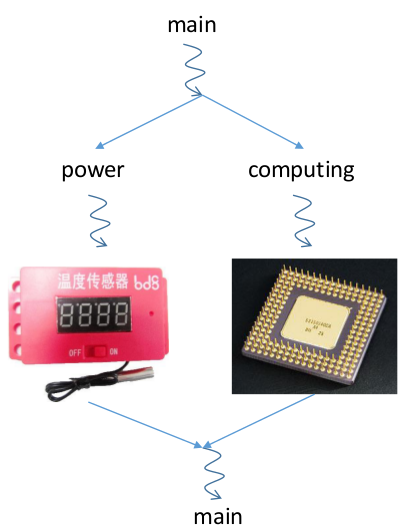
\includegraphics[height=3.14159in]{micgpupower}
  \caption{Power measurement on MIC and GPU}
\end{figure}

如果程序的运行时间很短,比如LTE PHY层模块运行一帧的时间就很短,甚至都无法达到时间窗口或和时间窗口在同一个数量级,我们就必须增加运行时间使其远大于时间窗口值,以使测得的energy值足够准确。

目前检测K20的power值只能在host端进行,所以我们用host端的一个进程通过调用NVIDIA提供的API来获取device端的power数据。这里有一个power值的threshold,只有device上的power值达到或超过这个threshold才进行采样,并在统计的同时累加采样时间,将这个时间称为device活动的时间(active time)。增加程序运行时间我们目前有两种思路:1)调用kernel多次;2)在kernel中让一个线程重复执行相同任务多次。思路1得到的时间是kernel运行一次时间的线性倍数,所以这个时间能够理想的模拟线性扩大kernel执行时间,但是这样做得到的active time要比kernel执行多次的时间累加值大,这可能是由于kernel的launch和retire引起的power上升时间,也被统计到了kernel执行时间中。对于第二种思路,由于GPU上线程调度,其实线性增加一个线程的执行时间并不意味着kernel执行时间的线性增加,但是由于kernel只被launch了一次,因此得到的active time和kernel的运行时间较为吻合;经过实验测试,这种方法测得的kernel执行时间与第一种方法通过多次调用kernel得到的时间相比得到的误差,要比第一种方法中active time和kernel执行多次得到的时间相比的差值要小很多。因此目前我们使用第二种思路来测量energy。另外,我们可以在第二种方法中的kernel中,在当一个线程重复执行相同任务的迭代之间加同步操作来进一步减小误差值,使得到的时间更接近kernel执行一次的线性倍数。

注意:即使只launch kernel,而kernel里什么也不做,这个launch的overhead相对于lte physical中这些模块的一次运行时间也比较大。

在MIC上,我们目前使用native模式运行程序,所以直接在device端使用一个监测sensor的线程,采样和统计的思路和GPU上的做法类似。不过说是监测sensor,其实是不断的读device上“/sys/class/micras/power”这个文件来获取其中的power数据,这个读文件的操作会给我们采样时间窗口增加误差。也就是说,我们的初衷是要让采样时间窗口的累加值和MIC上计算线程的运行时间大致相同,但是由于监测线程中除采样时间之外的其它开销(例如上述的读文件操作),使得线程的运行时间要大于采样时间的累加值,因此我们在最后计算energy时要适当修正采样时间窗口值,让每个时间窗口值加上这些其它操作的开销。

在测dft和fft的energy时,当数据集较小时(如dft的长度为75和150时),power的active time要比设计kernel的运行时间小不少,当数据集逐渐增大时,二者的差距逐渐减小趋近相等。我想这时因为数据集较小时,活动的线程数据较少,芯片上的能耗也较小;当活动线程数目随着数据集增多,能耗值也随之增大,采样power值超过threshold的次数越来越多。

\subsection{CPU}

在用20个线程运行Scrambling时,使用RAPL测量power和energy时得到的运行时间比不测power时测得的运行时间少一个数量级,这时不能用直接测得的时间求Performance per Watt,要用RAPL得到的那个时间,因为power是用RAPL算出来的。若出现这种情况要注意修正。

\subsection{TODO List}

\begin{verbatim}
amplxe-cl -collect knc-general-exploration -knob enable-vpu-metrics=true -knob enable-tlb-metrics=true -knob target-cards=0 -app-working-dir /home/xblee/ParWiBench/src/Equalizing/mic -app-working-dir /home/xblee/ParWiBench/src/Equalizing --search-dir all:rp=/home/xblee/ParWiBench/src/Equalizing/mic --search-dir all:rp=/home/xblee/ParWiBench/src/Equalizing -- ssh mic0 /home/xblee/ParWiBench/src/Equalizing/mic/CEEQ_all.out 0
\end{verbatim}

\bibliographystyle{plain}
\bibliography{../ref}

\end{document}


